\documentclass[11pt]{article}

% ---- Fonts (nice if available, graceful fallback) -------------------------- %
\usepackage[T1]{fontenc}
\usepackage[utf8]{inputenc}
\usepackage{amsmath}
\IfFileExists{newtxtext.sty}{%
  \usepackage{newtxtext}%
  \usepackage{newtxmath}%   % newtxmath also provides the AMS symbol set
}{%
  \usepackage{amssymb}%
  \usepackage{lmodern}%
}
\usepackage{microtype}

% ---- Layout & math --------------------------------------------------------- %
\usepackage[margin=1in]{geometry}
\usepackage{booktabs}
\usepackage{graphicx}
\usepackage{float}
\usepackage{caption}
\captionsetup{font=small,labelfont=bf}
\usepackage[round,authoryear]{natbib}
\usepackage[hidelinks]{hyperref}
\usepackage{xcolor}
\usepackage{enumitem}

\graphicspath{{../figures/}{figures/}}
% Auto-generated by src/run_all.py -- do not edit by hand.
\newcommand{\dataStart}{2000-01-03}
\newcommand{\dataEnd}{2026-04-30}
\newcommand{\nMonthly}{316}
\newcommand{\retRtwo}{-12.2\%}
\newcommand{\volRtwo}{28.1\%}
\newcommand{\sharpeBH}{0.48}
\newcommand{\sharpeManaged}{0.61}
\newcommand{\sharpeBest}{0.75}
\newcommand{\bestForecaster}{GARCH}
\newcommand{\sharpeBHcommon}{0.66}
\newcommand{\sharpeNaiveCommon}{0.60}
\newcommand{\annRetBH}{7.6\%}
\newcommand{\annRetManaged}{9.6\%}
\newcommand{\maxddBH}{-54.2\%}
\newcommand{\maxddManaged}{-42.9\%}
\newcommand{\alphaManaged}{3.6\%}
\newcommand{\alphaTstat}{1.89}
\newcommand{\appraisal}{0.37}
\newcommand{\betaManaged}{0.78}
\newcommand{\alphaUncapped}{3.4\%}
\newcommand{\alphaUncappedT}{1.22}
\newcommand{\deflatedSharpe}{0.999}
\newcommand{\breakevenCost}{39}
\newcommand{\nAssets}{11}
\newcommand{\sharpeDivBH}{0.39}
\newcommand{\sharpeDivManaged}{0.41}
\newcommand{\sharpeDivTrend}{0.72}
\newcommand{\maxddDivBH}{-45.0\%}
\newcommand{\maxddDivTrend}{-23.9\%}
\newcommand{\alphaDivTrend}{8.0\%}
\newcommand{\alphaDivTrendT}{3.63}
\newcommand{\sharpeDivTrendNet}{0.64}
\newcommand{\costBpsExt}{10}
   % auto-generated numbers (\sharpeManaged, ...)

% Interactive companion site. Replace with your deployed URL (e.g. GitHub Pages).
\newcommand{\siteurl}{https://your-deployment-url}

\setlength{\parskip}{0.4em}
\setlength{\parindent}{0pt}

\title{\textbf{Trade the Risk, Not the Price}\\[4pt]
  {\large Volatility Timing, Trend, and Regimes Across Global Markets}}
\author{Clément Bellet-Odent}
\date{\today}

\begin{document}
\maketitle

\begin{center}
\fcolorbox{black!12}{blue!5}{%
  \parbox{0.93\linewidth}{\centering\small
  \textbf{Interactive companion.} To experiment with this research from another
  angle --- choosing the asset, the volatility forecaster, the leverage cap and
  the trading cost, and watching the Sharpe ratio, returns and drawdowns
  recompute \emph{live} in your browser --- open the interactive lab
  (\texttt{site/index.html}) or visit \url{\siteurl}.}}
\end{center}
\vspace{4pt}

% =========================================================================== %
\begin{abstract}
\noindent
The direction of stock returns is essentially unpredictable, but their
\emph{risk} is not. We exploit this asymmetry by replicating the
volatility-managed strategy of \citet{moreira2017volatility} on the US market
factor (\dataStart{} to \dataEnd, \nMonthly{} months from the Ken French Data
Library), scaling market exposure by the inverse of a one-month-ahead variance
forecast and normalising to the volatility of buy-and-hold. Out of sample, the
prevailing-mean benchmark beats every return-forecasting model (R\textsuperscript{2}
of \retRtwo), while volatility is strongly forecastable (R\textsuperscript{2} of
\volRtwo). The managed strategy lifts the annualised Sharpe ratio from
\sharpeBH{} to \sharpeManaged{} (a \bestForecaster{} forecaster lifts it further,
to \sharpeBest{} on the common 2004--2026 sample), cuts the maximum drawdown from
\maxddBH{} to \maxddManaged, and
earns an annualised alpha of \alphaManaged{} ($t=\alphaTstat$). The result
survives a Deflated Sharpe Ratio of \deflatedSharpe{} (correcting for multiple
testing and non-normality) and transaction costs up to roughly \breakevenCost{}
bps. A Hidden Markov Model, given only returns and no crisis dates, rediscovers
the turbulent regimes and shows the mechanism: the strategy levers up in calm
markets and de-risks in turbulent ones, trading away some violent-rebound upside
for materially lower drawdowns. Extending to a panel of \nAssets{} assets across
four classes, simple volatility timing does \emph{not} travel uniformly --- it is
largely an equity-index phenomenon --- but a diversified, risk-parity portfolio
that adds a time-series-momentum overlay lifts the Sharpe ratio from \sharpeDivBH{}
(diversified buy-and-hold) to \sharpeDivTrend, halves the drawdown
(\maxddDivBH{} to \maxddDivTrend), earns an annualised alpha of \alphaDivTrend{}
($t=\alphaDivTrendT$), and stays at \sharpeDivTrendNet{} net of \costBpsExt-bps
costs. This is a research study, not investment advice.
\end{abstract}

% =========================================================================== %
\section{Introduction}

A central prediction of efficient markets is that the \emph{direction} of returns
is close to unpredictable: if it were not, the trade would already have been put
on. Decades of out-of-sample evidence bear this out \citep{campbell2008predicting}.
Yet a second, equally robust fact sits alongside it: return \emph{variance} is
highly persistent and forecastable, the phenomenon of volatility clustering first
modelled by \citet{engle1982autoregressive} and \citet{bollerslev1986generalized}.

\citet{moreira2017volatility} turn this asymmetry into a portfolio rule. Because
high realized variance this month predicts high variance next month, but not low
returns next month, an investor who scales down exposure when variance is high
(and up when it is low) earns a higher Sharpe ratio than a static position in the
same asset. The result is striking precisely because it does not require
predicting returns at all.

This paper makes four contributions. First, a \textbf{clean, fully reproducible
replication} on the post-2000 US market factor, with every number regenerated
from source by a single command. Second, an emphasis on the \textbf{rigour that
distinguishes a credible backtest}: strictly out-of-sample (walk-forward)
volatility forecasts, the QLIKE loss \citep{patton2011volatility} and
Diebold--Mariano tests \citep{diebold1995comparing} for forecast comparison,
explicit transaction costs and leverage caps, and the Deflated Sharpe Ratio
\citep{bailey2014deflated} to pre-empt the data-mining objection. Third, a
\textbf{regime-based explanation} layer: a Hidden Markov Model
\citep{hamilton1989new} that, with no crisis dates supplied, recovers the
turbulent periods and lets us decompose \emph{where} the edge is earned. Fourth, a
\textbf{multi-asset robustness test and a trend overlay}: we run the strategy
across \nAssets{} assets in four classes and show that, while volatility timing
alone does not travel uniformly, combining it with time-series momentum
\citep{moskowitz2012time} in a diversified portfolio produces a markedly stronger
and more significant result.

We are deliberately honest about magnitudes. On this particular sample --- which
contains two unusually fast crashes (2020, and the 2022 repricing) --- the naive
estimator's edge is real but modest and inherits fat left tails when leverage is
left uncapped; it strengthens with a sensible leverage cap and a better variance
forecast. We view stating this plainly as part of the contribution.

% =========================================================================== %
\section{Background and Literature}

\textbf{Volatility forecasting.} ARCH/GARCH models
\citep{engle1982autoregressive,bollerslev1986generalized} capture conditional
heteroskedasticity through a recursion in past squared shocks and past variance.
The Heterogeneous Autoregressive (HAR) model of \citet{corsi2009simple}
regresses realized variance on its own short-, medium- and long-horizon averages
and is a strong, parsimonious benchmark, especially with realized-variance data
\citep{andersen2003modeling}. Comparing volatility forecasts is subtle because
the target is latent; \citet{patton2011volatility} shows that the QLIKE and MSE
losses are robust to noise in the volatility proxy, and
\citet{diebold1995comparing}, with the small-sample correction of
\citet{harvey1997testing}, provide the test of equal predictive accuracy.

\textbf{Volatility management.} \citet{moreira2017volatility} document that
scaling factor exposure by inverse realized variance raises Sharpe ratios across
equity factors and internationally. \citet{cederburg2020economic} provide a
careful, more sceptical out-of-sample appraisal, motivating exactly the
robustness checks we run here.

\textbf{Return (un)predictability.} \citet{campbell2008predicting} formalise the
out-of-sample R\textsuperscript{2} against the prevailing mean, and
\citet{clark2007approximately} give the appropriate test for nested models. We
use both to establish the null result.

\textbf{Multiple testing.} \citet{bailey2012sharpe,bailey2014deflated} derive the
Probabilistic and Deflated Sharpe Ratios, which adjust an observed Sharpe ratio
for sample length, skewness/kurtosis and the number of configurations tried.

\textbf{Regimes.} \citet{hamilton1989new} introduced Markov-switching models to
finance; a Gaussian HMM is the natural unsupervised tool for discovering
calm/turbulent states from returns alone.

% =========================================================================== %
\section{Data}

We use daily research factors from the Ken French Data Library: the market excess
return \texttt{Mkt-RF} and the risk-free rate \texttt{RF}. Working in excess
returns from the outset makes Sharpe ratios correct by construction. The sample
runs \dataStart{} to \dataEnd. We aggregate to monthly excess returns by
compounding, and define monthly \textbf{realized variance} as the sum of squared
daily excess returns within the month,
\(\mathrm{RV}_t=\sum_{d\in t} r_d^2\), the standard daily-data proxy. Table
\ref{tab:descriptive} reports descriptive statistics; the well-known negative
skewness and excess kurtosis of equity returns are visible and motivate the
robust evaluation tools used below.

\begin{table}[htbp]
\centering
\caption{Descriptive statistics, US market excess return (Ken French).}
\label{tab:descriptive}
\small
\begin{tabular}{lrr}
\toprule
Statistic & Daily Mkt-RF & Monthly Mkt-RF \\
\midrule
N obs & 6621.0000 & 316.0000 \\
Ann. mean & 0.0810 & 0.0743 \\
Ann. vol & 0.1961 & 0.1577 \\
Sharpe & 0.4132 & 0.4711 \\
Skewness & -0.1680 & -0.4706 \\
Excess kurtosis & 9.3296 & 0.7666 \\
Min & -0.1201 & -0.1721 \\
Max & 0.1136 & 0.1362 \\
\bottomrule
\end{tabular}
\end{table}


% =========================================================================== %
\section{Methodology}

\subsection{Volatility forecasting and out-of-sample evaluation}

The target is next month's realized variance. We compare four one-step-ahead
forecasters, all evaluated \textbf{walk-forward} on an expanding window so that a
forecast for month $t+1$ uses only information available at the end of month $t$:

\begin{enumerate}[leftmargin=1.4em,itemsep=0.1em]
  \item \textbf{Naive (random walk):} $\widehat{\mathrm{RV}}_{t+1}=\mathrm{RV}_t$
        --- the exact estimator in \citet{moreira2017volatility}.
  \item \textbf{GARCH(1,1):} fit on daily excess returns up to the end of month
        $t$; the analytic 1-to-$H$ day-ahead variance forecasts are summed to a
        monthly variance.
  \item \textbf{HAR:} a monthly heterogeneous autoregression with 1-, 3- and
        12-month realized-variance components \citep{corsi2009simple}, fit by
        expanding-window OLS.
  \item \textbf{Ensemble:} the mean of the GARCH and HAR forecasts.
\end{enumerate}

Accuracy is measured by RMSE and by the proxy-robust \textbf{QLIKE} loss
\citep{patton2011volatility},
\(\mathrm{QLIKE}=\tfrac1N\sum_t\big(\tfrac{\mathrm{RV}_t}{h_t}-\log\tfrac{\mathrm{RV}_t}{h_t}-1\big)\),
where $h_t$ is the forecast. Differences are tested with the Diebold--Mariano
statistic using the \citet{harvey1997testing} small-sample correction.

\subsection{Strategy construction and the volatility normalisation}

The managed excess return scales next month's market return by inverse forecast
variance,
\begin{equation}
  f^{\text{managed}}_{t} \;=\; \frac{c}{\widehat{\sigma}^2_{t}}\, f_{t},
  \label{eq:managed}
\end{equation}
where $f_t$ is the market excess return in month $t$ and $\widehat{\sigma}^2_t$
is the variance forecast for month $t$ formed at the end of month $t-1$. Calm
markets imply low forecast variance and therefore large exposure; nervous markets
imply de-risking.

The constant $c$ is chosen so that the managed series has the \textbf{same
full-sample volatility as buy-and-hold}. This normalisation is not optional: a
Sharpe-ratio comparison is only meaningful at equal risk. Because $c$ is a single
scalar, it leaves the Sharpe ratio and the regression $t$-statistics below
unchanged; the time-varying \emph{weights} use only past information. We report
the headline strategy with the naive forecaster and a realistic $2\times$
leverage cap (an a-priori risk limit, not chosen to maximise performance), and
separately show the effect of better forecasters and of the cap.

\subsection{The Hidden Markov regime layer}

We fit a two-state Gaussian HMM to monthly returns; states are relabelled by
variance (calm, turbulent). We draw a sharp methodological line. \emph{Smoothed}
(full-sample) state probabilities are used only to \emph{describe and visualise}
the regime structure --- legitimate because it is descriptive, not a trading
decision. If a regime signal were used inside the backtest, only \emph{filtered}
(online) inference would be admissible; we implement it by refitting the HMM
walk-forward and taking the end-point posterior (which, having no future data,
equals the filtered probability). Using smoothed states to trade would be
lookahead bias. The strategy in \eqref{eq:managed} is \emph{not}
regime-conditioned; the HMM serves only to explain the result.

% =========================================================================== %
\section{Results}

\subsection{The null result: return vs.\ volatility}

Figure \ref{fig:r2} and Table \ref{tab:predictability} make the framing point.
Every model that forecasts next month's \emph{return} has a \emph{negative}
out-of-sample R\textsuperscript{2} (worse than the prevailing mean; the
Clark--West statistics confirm no significant improvement). Forecasting next
month's \emph{volatility} yields R\textsuperscript{2} around \volRtwo. The
direction of prices is noise; their risk is not.

\begin{figure}[H]\centering
  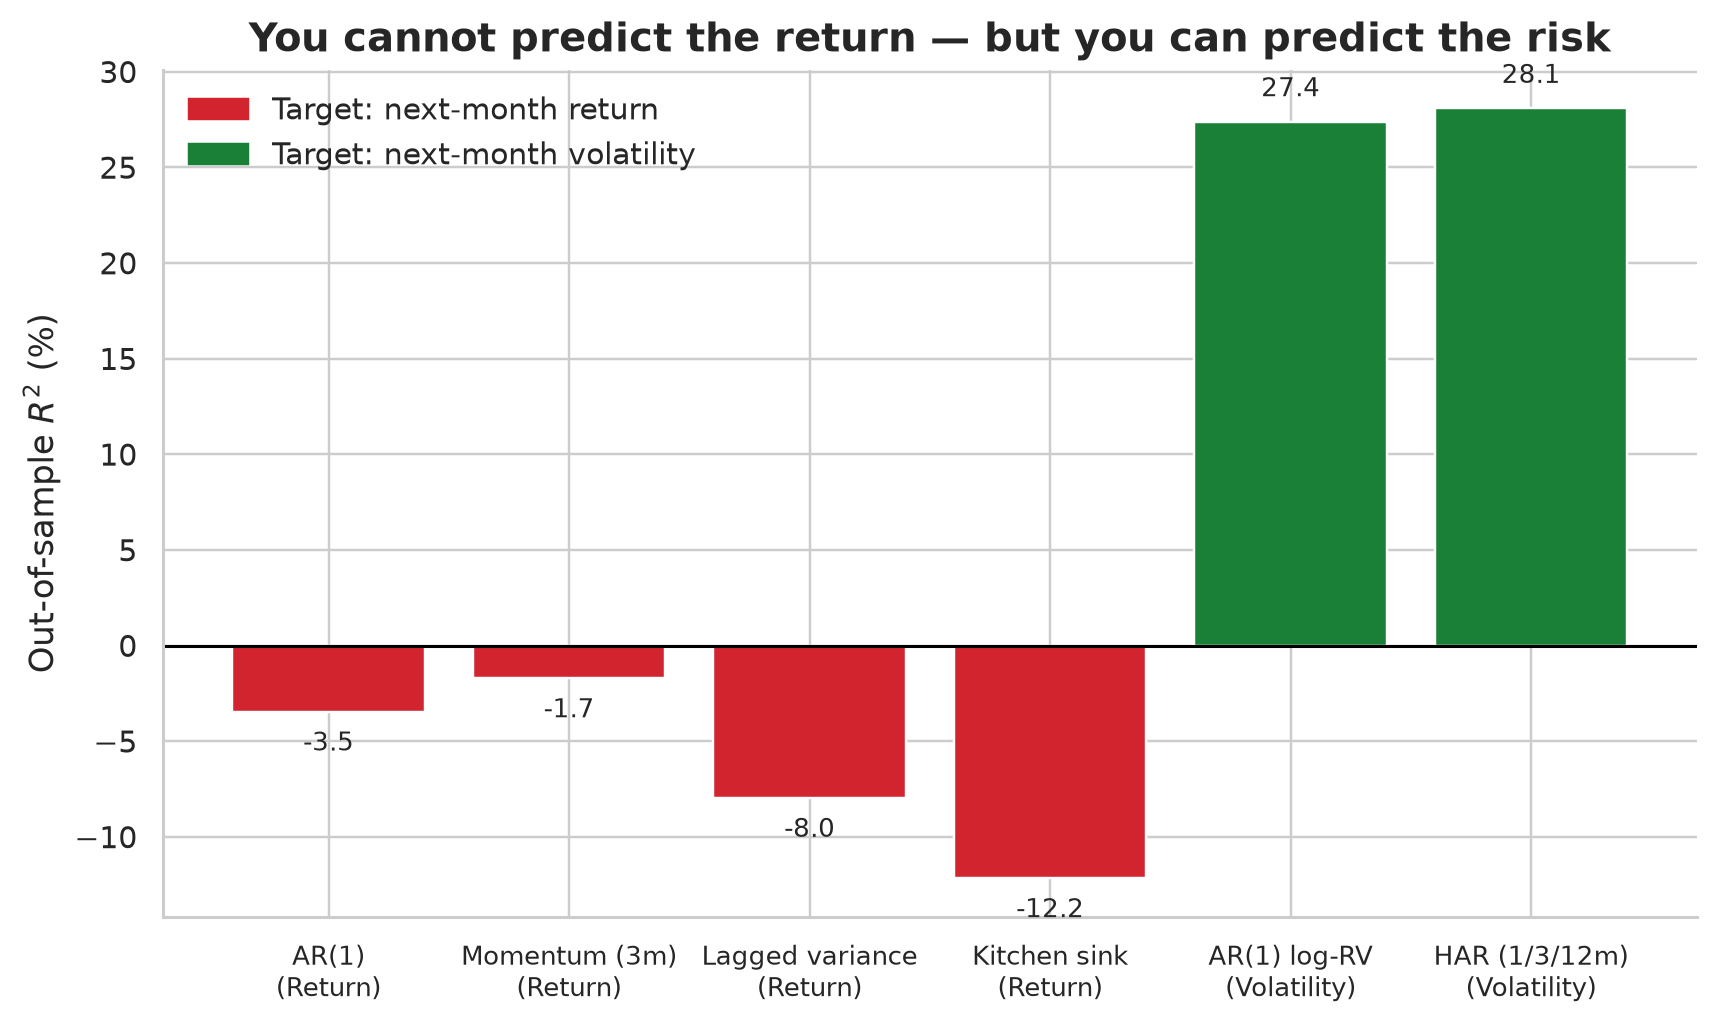
\includegraphics[width=0.86\textwidth]{fig01_predictability_r2.png}
  \caption{Out-of-sample R\textsuperscript{2} against the prevailing mean.
  Forecasting the return fails; forecasting the volatility succeeds.}
  \label{fig:r2}
\end{figure}

\begin{table}[htbp]
\centering
\caption{Out-of-sample $R^2$: forecasting the return vs forecasting the volatility (expanding window, vs the prevailing mean).}
\label{tab:predictability}
\small
\begin{tabular}{llrrr}
\toprule
Target & Model & R2\_OOS & CW\_stat & CW\_pvalue \\
\midrule
Return & AR(1) & -0.0345 & -1.5133 & 0.9349 \\
Return & Momentum (3m) & -0.0171 & -1.1259 & 0.8699 \\
Return & Lagged variance & -0.0796 & -0.7453 & 0.7719 \\
Return & Kitchen sink & -0.1216 & -1.0460 & 0.8522 \\
Volatility (log-RV) & AR(1) log-RV & 0.2740 & -- & -- \\
Volatility (log-RV) & HAR (1/3/12m) & 0.2810 & -- & -- \\
\bottomrule
\end{tabular}
\end{table}


\subsection{Which volatility forecaster wins}

Table \ref{tab:volmetrics} reports RMSE and QLIKE on the common evaluation
sample; Table \ref{tab:dm} the Diebold--Mariano tests. GARCH is the most accurate
forecaster, significantly beating the naive benchmark on QLIKE
(Figure \ref{fig:volfc} shows its one-step-ahead forecast tracking realized
volatility, including the 2008 and 2020 spikes).

\begin{table}[htbp]
\centering
\caption{Volatility-forecast accuracy (RMSE and QLIKE, common sample).}
\label{tab:volmetrics}
\small
\begin{tabular}{lrr}
\toprule
Model & RMSE & QLIKE \\
\midrule
naive & 0.00672 & 0.50566 \\
har & 0.00689 & 0.36184 \\
garch & 0.00536 & 0.28954 \\
ensemble & 0.00594 & 0.31259 \\
\bottomrule
\end{tabular}
\end{table}

\begin{table}[htbp]
\centering
\caption{Diebold-Mariano tests of equal predictive accuracy (HLN small-sample correction).}
\label{tab:dm}
\small
\begin{tabular}{llrrl}
\toprule
Comparison & Loss & DM\_stat & p\_value & better \\
\midrule
garch vs naive & RMSE/MSE & -1.596 & 0.112 & garch \\
garch vs naive & QLIKE & -3.376 & 0.001 & garch \\
har vs naive & RMSE/MSE & 0.258 & 0.797 & naive \\
har vs naive & QLIKE & -2.209 & 0.028 & har \\
ensemble vs naive & RMSE/MSE & -1.196 & 0.233 & ensemble \\
ensemble vs naive & QLIKE & -3.033 & 0.003 & ensemble \\
har vs garch & RMSE/MSE & 1.873 & 0.062 & garch \\
har vs garch & QLIKE & 2.497 & 0.013 & garch \\
\bottomrule
\end{tabular}
\end{table}


\begin{figure}[H]\centering
  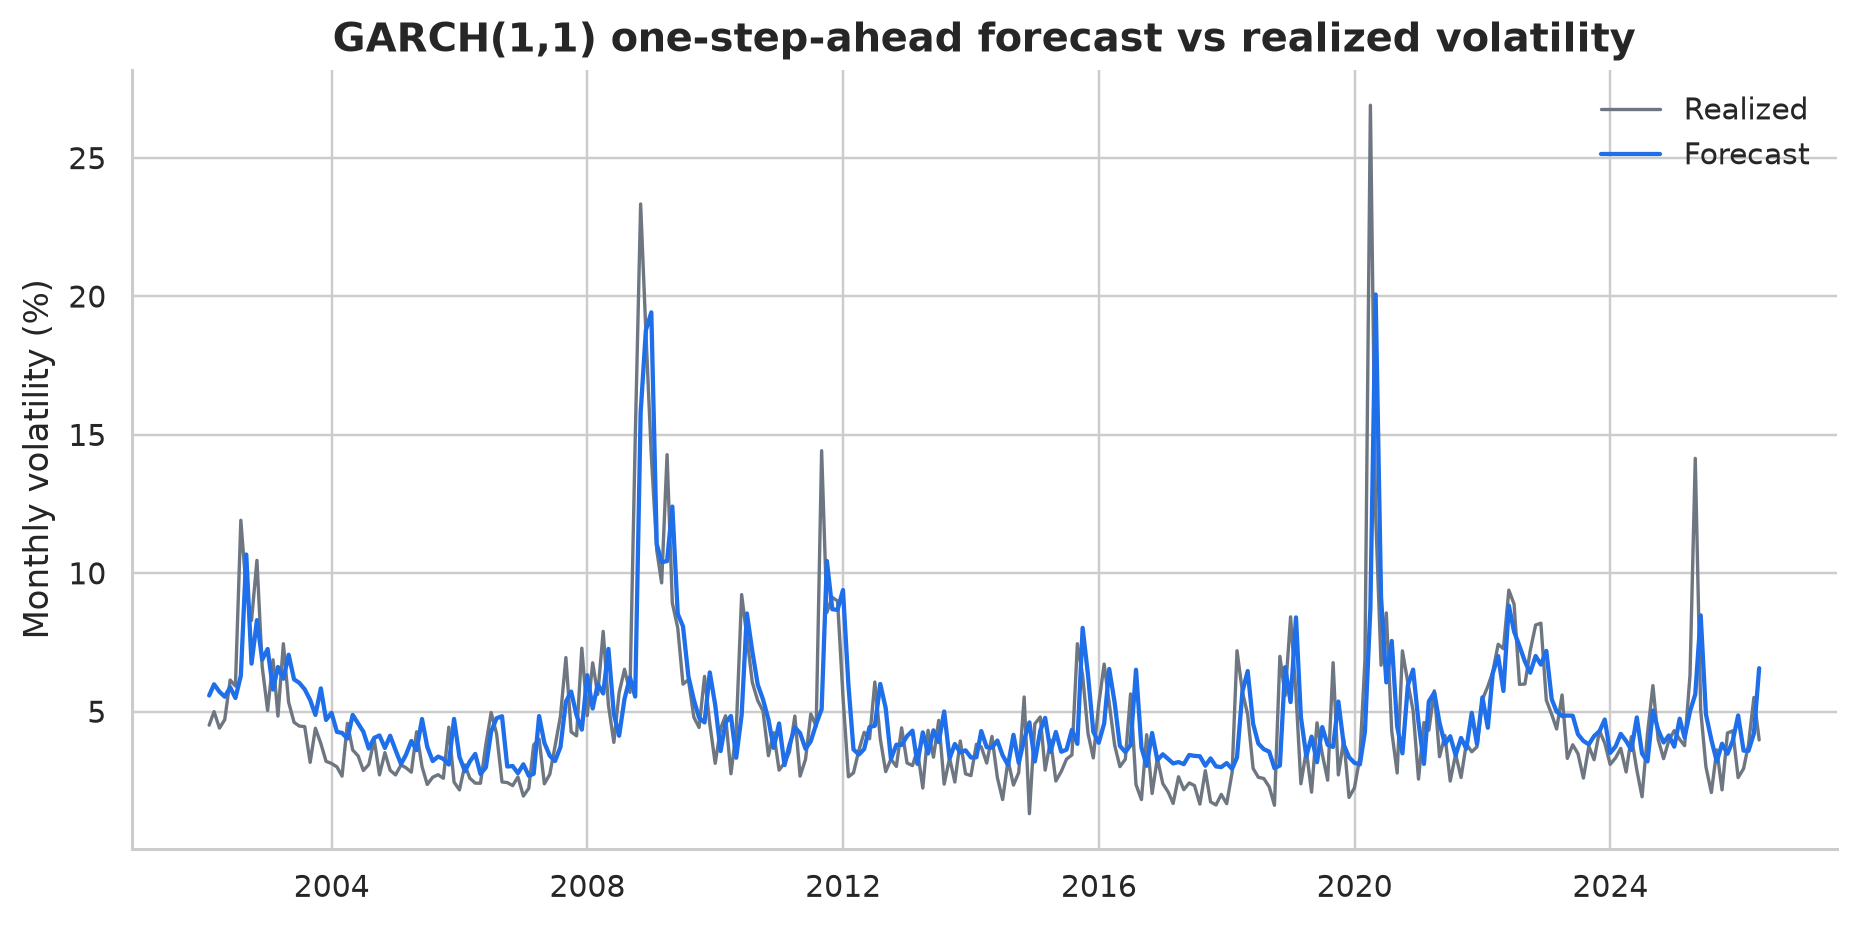
\includegraphics[width=0.92\textwidth]{fig02_vol_forecast.png}
  \caption{GARCH(1,1) one-step-ahead forecast vs.\ realized monthly volatility,
  walk-forward.}
  \label{fig:volfc}
\end{figure}

\subsection{Strategy performance}

The managed exposure (Figure \ref{fig:exposure}) levers up in calm periods and
cuts risk in turbulent ones. Over the full sample the strategy raises the Sharpe
ratio from \sharpeBH{} to \sharpeManaged, lifts the annualised return from
\annRetBH{} to \annRetManaged{} at matched volatility, and reduces the maximum
drawdown from \maxddBH{} to \maxddManaged{} (Table \ref{tab:metrics},
Figure \ref{fig:equity}). Regressing the managed series on the market gives an
annualised alpha of \alphaManaged{} ($t=\alphaTstat$, Newey--West) with an
appraisal ratio of \appraisal. On the common evaluation sample where every
forecaster is available (uncapped), switching from the naive to the more accurate
\bestForecaster{} forecaster raises the Sharpe ratio from \sharpeNaiveCommon{} to
\sharpeBest{} (Table \ref{tab:forecasters}).

\begin{figure}[H]\centering
  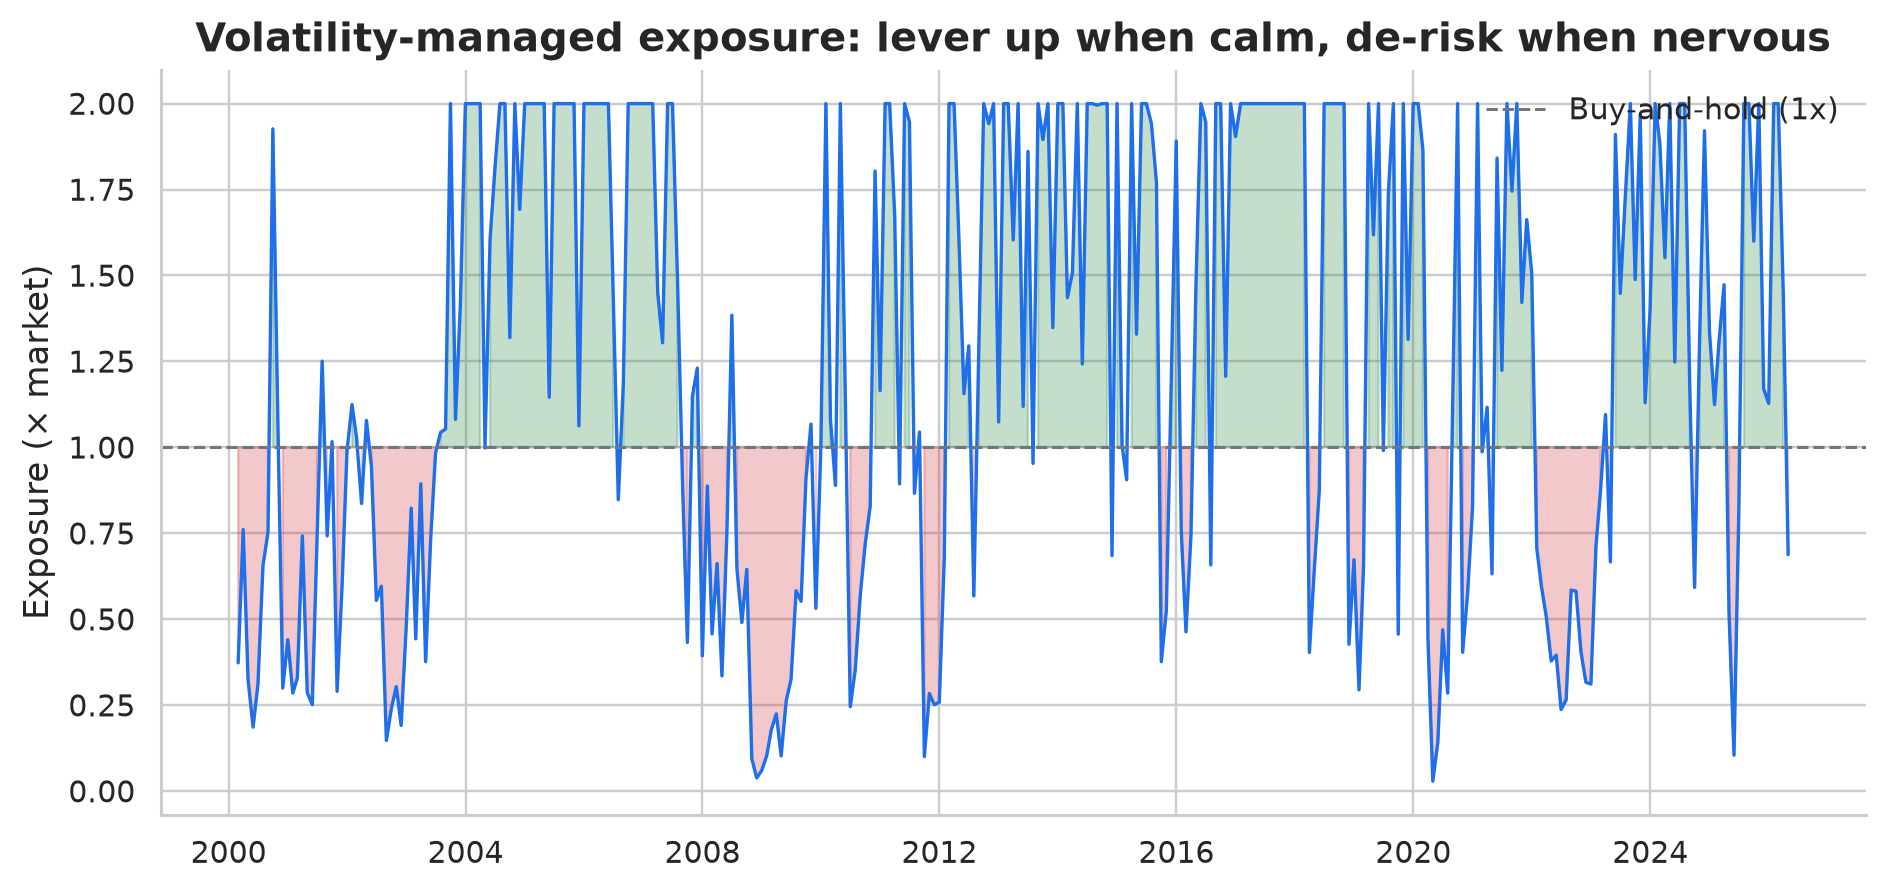
\includegraphics[width=0.92\textwidth]{fig04_exposure.png}
  \caption{Time-varying exposure of the volatility-managed strategy.}
  \label{fig:exposure}
\end{figure}

\begin{table}[htbp]
\centering
\caption{Headline performance: volatility-managed (naive forecast, 2$\times$ cap) vs buy-and-hold, vol-matched.}
\label{tab:metrics}
\small
\begin{tabular}{lrr}
\toprule
Metric & buy\_and\_hold & managed\_headline \\
\midrule
ann\_return & 0.076 & 0.096 \\
cagr & 0.066 & 0.087 \\
ann\_vol & 0.158 & 0.158 \\
sharpe & 0.484 & 0.610 \\
sortino & 0.705 & 0.910 \\
max\_drawdown & -0.542 & -0.429 \\
calmar & 0.121 & 0.202 \\
skew & -0.479 & -0.539 \\
excess\_kurtosis & 0.789 & 0.777 \\
n\_months & 315.000 & 315.000 \\
\bottomrule
\end{tabular}
\end{table}


\begin{figure}[H]\centering
  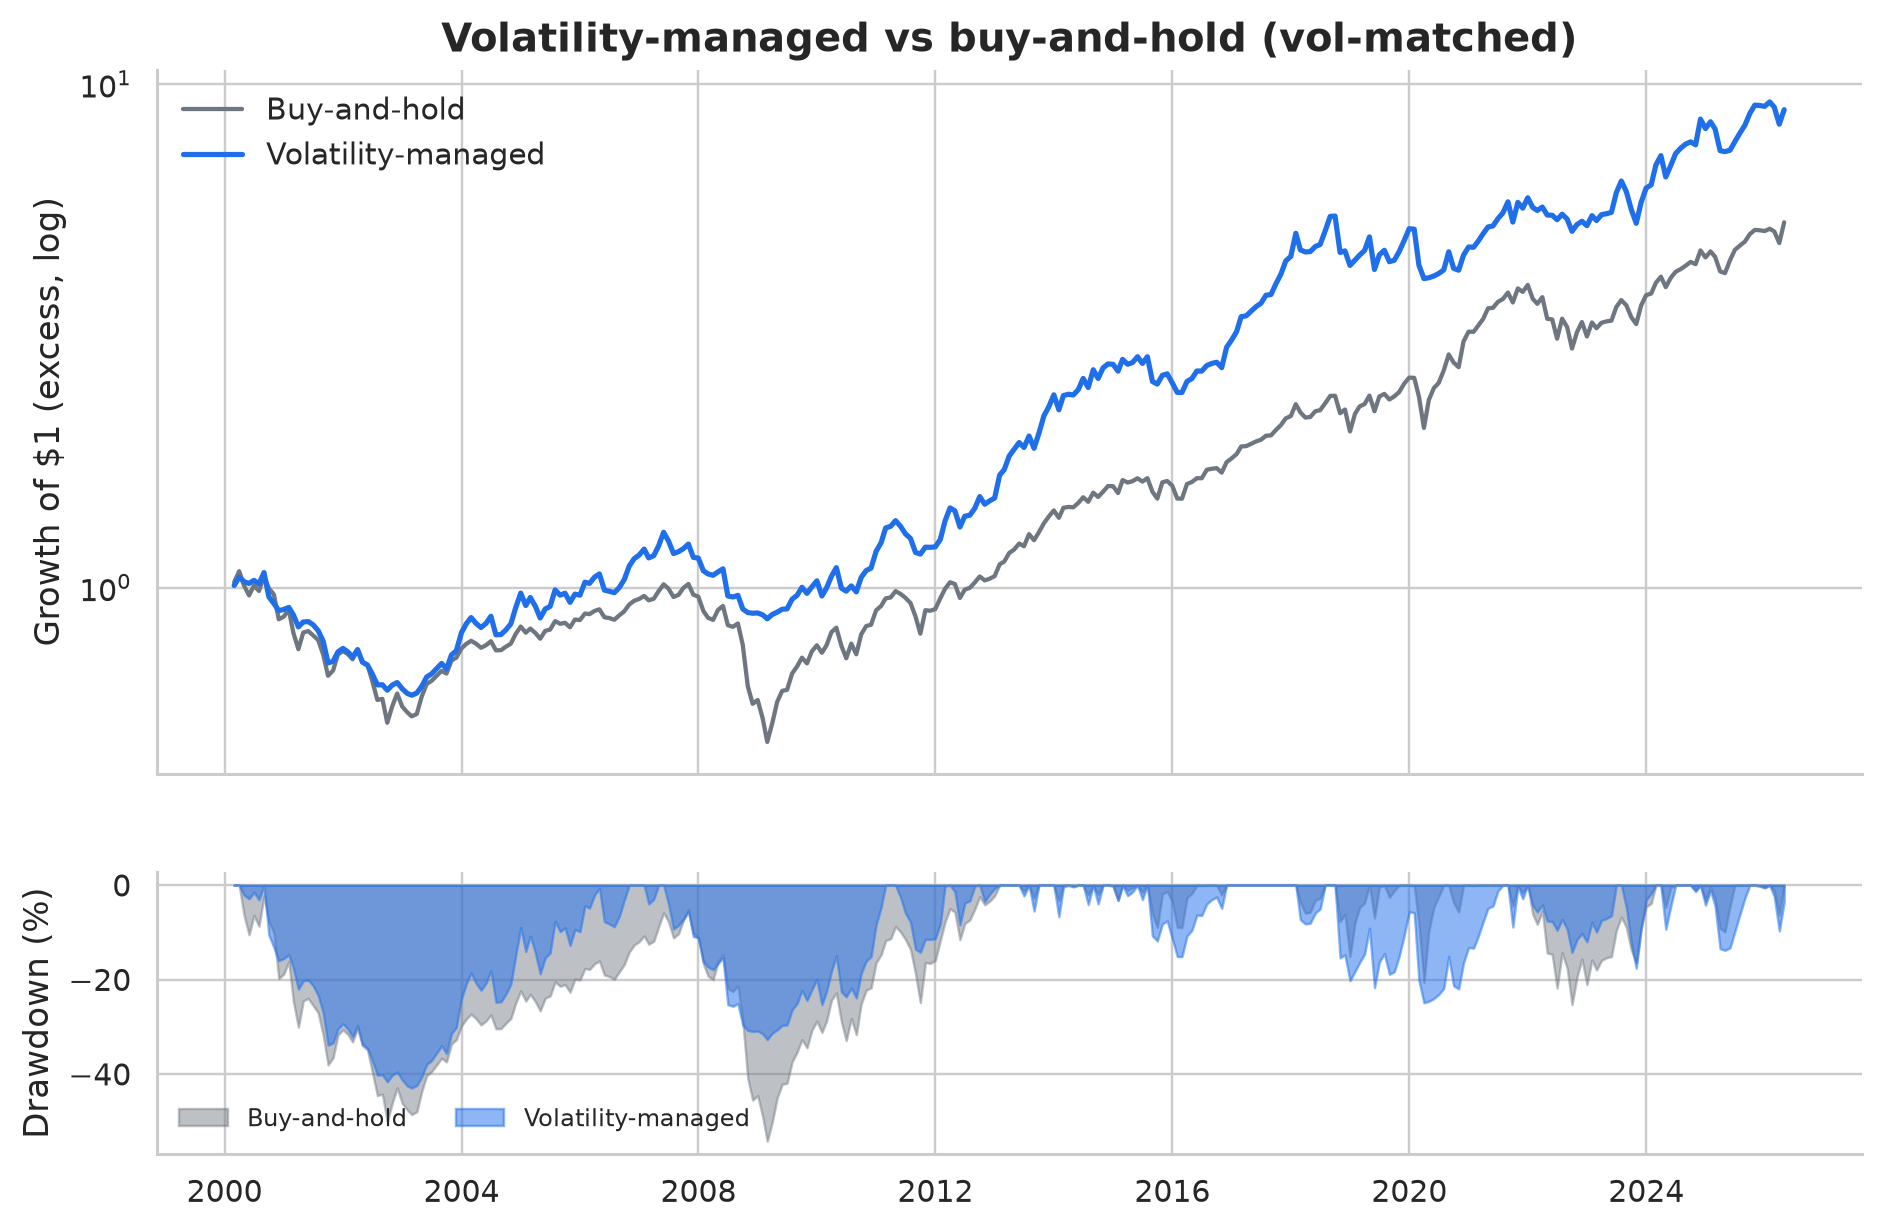
\includegraphics[width=0.92\textwidth]{fig05_equity_curve.png}
  \caption{Growth of \$1 in excess returns (log scale) and drawdowns, managed
  vs.\ buy-and-hold at matched full-sample volatility.}
  \label{fig:equity}
\end{figure}

\begin{table}[htbp]
\centering
\caption{Managed-strategy performance by volatility forecaster (common sample, uncapped).}
\label{tab:forecasters}
\small
\begin{tabular}{lrrrrrrr}
\toprule
forecaster & ann\_return & ann\_vol & sharpe & max\_drawdown & alpha\_annual & alpha\_tstat & appraisal\_ratio \\
\midrule
naive & 0.090 & 0.151 & 0.597 & -0.442 & 0.030 & 0.966 & 0.248 \\
har & 0.108 & 0.151 & 0.715 & -0.355 & 0.026 & 1.263 & 0.307 \\
garch & 0.113 & 0.151 & 0.747 & -0.327 & 0.035 & 1.561 & 0.374 \\
ensemble & 0.111 & 0.151 & 0.735 & -0.337 & 0.031 & 1.433 & 0.348 \\
buy\_and\_hold & 0.099 & 0.151 & 0.655 & -0.514 & 0.000 & -- & -- \\
\bottomrule
\end{tabular}
\end{table}


% =========================================================================== %
\section{Robustness}

\textbf{Transaction costs.} The strategy retrades as the leverage target moves.
Charging a proportional cost on turnover (Table \ref{tab:costs},
Figure \ref{fig:costs}), the edge survives up to a break-even of roughly
\breakevenCost{} bps per unit of turnover --- comfortably above realistic costs
for a liquid index exposure.

\textbf{Leverage cap.} Uncapped, the naive strategy occasionally takes large
positions and inherits fat left tails; the literal \citet{moreira2017volatility}
estimator without a cap earns an alpha of \alphaUncapped{} ($t=\alphaUncappedT$).
Capping exposure at $1.5$--$3\times$ and re-normalising volatility both controls
the tails and improves risk-adjusted performance (Table \ref{tab:leverage}),
which is why the headline uses a $2\times$ cap.

\textbf{Sub-periods.} Table \ref{tab:subperiods} splits the sample. The strategy
helps most in turbulent, mean-reverting drawdowns and gives back some ground in
sharp high-volatility rebounds --- consistent with the regime decomposition below.

\begin{table}[htbp]
\centering
\caption{Transaction-cost sensitivity of the headline strategy.}
\label{tab:costs}
\small
\begin{tabular}{rrrrrr}
\toprule
cost\_bps & avg\_turnover & ann\_return & sharpe & alpha\_annual & alpha\_tstat \\
\midrule
0 & 0.418 & 0.096 & 0.610 & 0.036 & 1.889 \\
1 & 0.418 & 0.096 & 0.606 & 0.036 & 1.862 \\
2 & 0.418 & 0.095 & 0.603 & 0.035 & 1.835 \\
5 & 0.418 & 0.094 & 0.594 & 0.034 & 1.753 \\
10 & 0.418 & 0.091 & 0.578 & 0.031 & 1.617 \\
20 & 0.418 & 0.086 & 0.546 & 0.026 & 1.348 \\
\bottomrule
\end{tabular}
\end{table}

\begin{table}[htbp]
\centering
\caption{Leverage-cap sensitivity (volatility re-normalised within each cap).}
\label{tab:leverage}
\small
\begin{tabular}{rrrrrrrr}
\toprule
leverage\_cap & mean\_weight & max\_weight & ann\_return & ann\_vol & sharpe & alpha\_annual & alpha\_tstat \\
\midrule
1.000 & 1.000 & 1.000 & 0.076 & 0.158 & 0.484 & 0.000 & -- \\
1.500 & 1.191 & 1.500 & 0.096 & 0.158 & 0.612 & 0.031 & 1.850 \\
2.000 & 1.259 & 2.000 & 0.096 & 0.158 & 0.610 & 0.036 & 1.889 \\
3.000 & 1.244 & 3.000 & 0.094 & 0.158 & 0.593 & 0.040 & 1.764 \\
inf & 1.097 & 7.552 & 0.081 & 0.158 & 0.512 & 0.034 & 1.225 \\
\bottomrule
\end{tabular}
\end{table}


\begin{figure}[H]\centering
  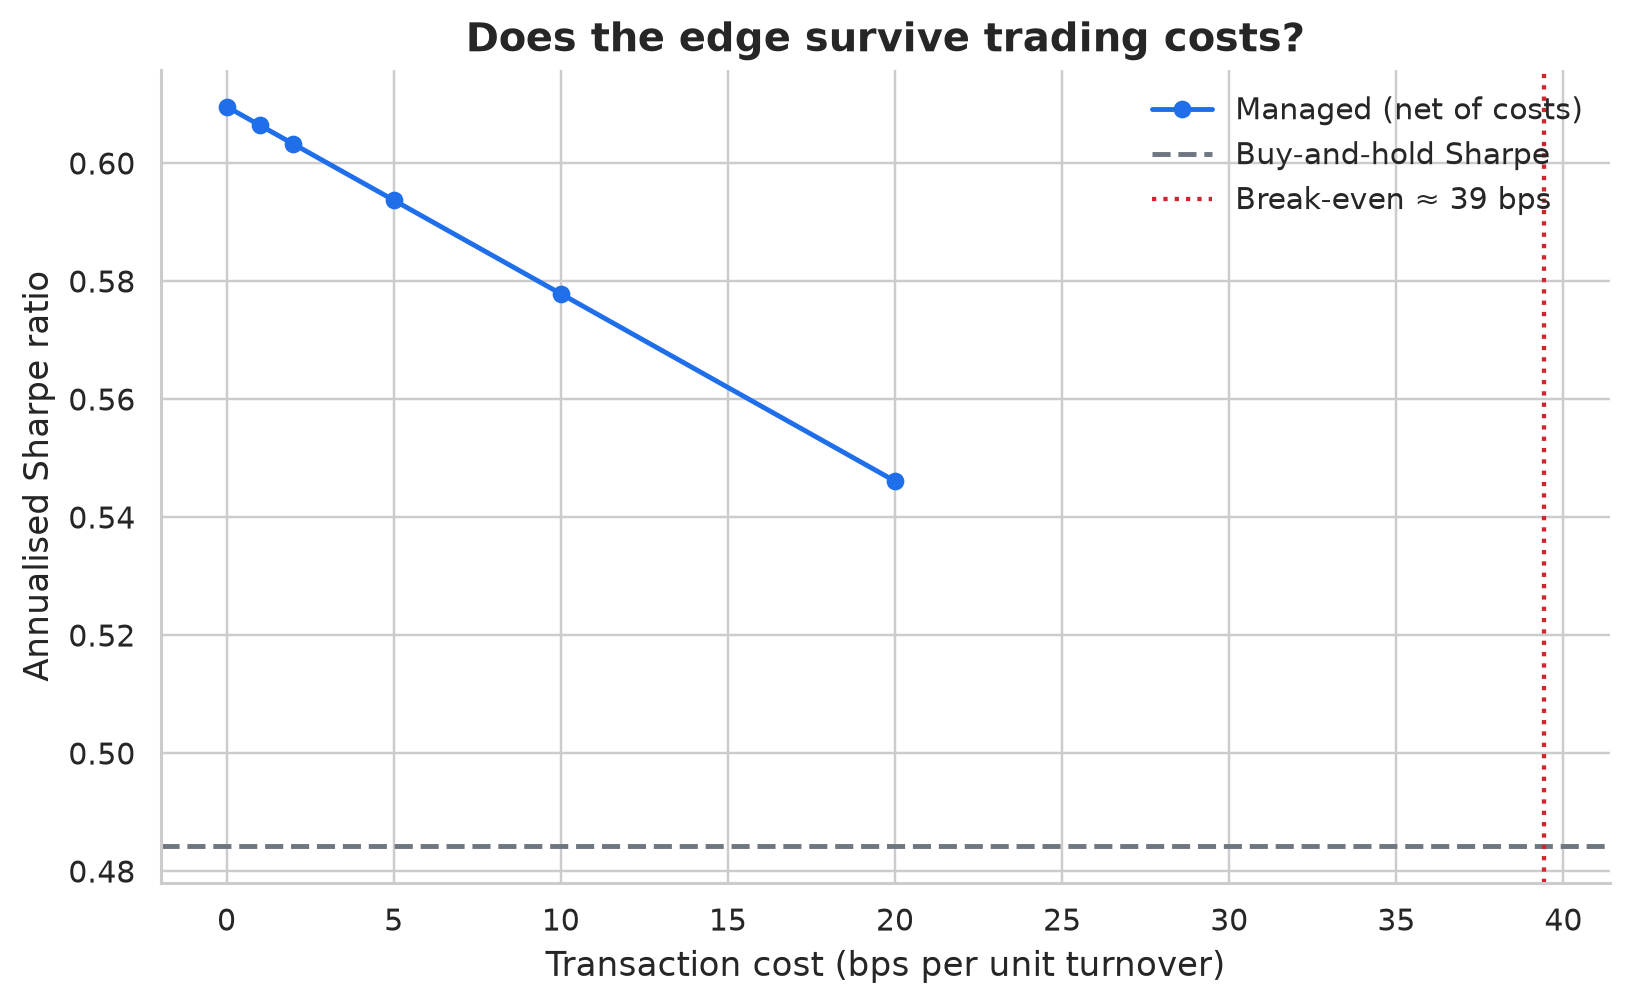
\includegraphics[width=0.7\textwidth]{fig06_cost_sensitivity.png}
  \caption{Net Sharpe ratio vs.\ transaction cost, with the break-even level.}
  \label{fig:costs}
\end{figure}

\begin{table}[htbp]
\centering
\caption{Sub-period analysis: managed vs buy-and-hold.}
\label{tab:subperiods}
\small
\begin{tabular}{lllrrrrrr}
\toprule
period & start & end & n & bh\_return & bh\_sharpe & mm\_return & mm\_sharpe & sharpe\_gain \\
\midrule
Dot-com bust & 2000-02-29 & 2002-12-31 & 35 & -0.166 & -0.844 & -0.150 & -1.212 & -0.368 \\
Mid-2000s calm & 2003-01-31 & 2007-06-30 & 54 & 0.124 & 1.398 & 0.160 & 1.188 & -0.210 \\
Global Financial Crisis & 2007-07-31 & 2009-06-30 & 24 & -0.205 & -0.914 & -0.147 & -1.260 & -0.346 \\
Post-GFC bull & 2009-07-31 & 2019-12-31 & 126 & 0.145 & 1.117 & 0.180 & 1.113 & -0.004 \\
COVID crash \& rebound & 2020-01-31 & 2020-12-31 & 12 & 0.247 & 0.893 & -0.059 & -0.263 & -1.156 \\
Post-COVID & 2021-01-31 & 2026-04-30 & 64 & 0.106 & 0.680 & 0.132 & 0.789 & 0.109 \\
\bottomrule
\end{tabular}
\end{table}


% =========================================================================== %
\section{Regime Analysis}

Given only monthly returns and \emph{no} crisis dates, the Gaussian HMM recovers
the turbulent regimes --- dot-com, the Global Financial Crisis, COVID-19 and the
2022 repricing all fall in the high-variance state (Figure \ref{fig:regimes},
Table \ref{tab:regimestats}). This is unsupervised structure discovery, not
curve-fitting to known events.

\begin{figure}[H]\centering
  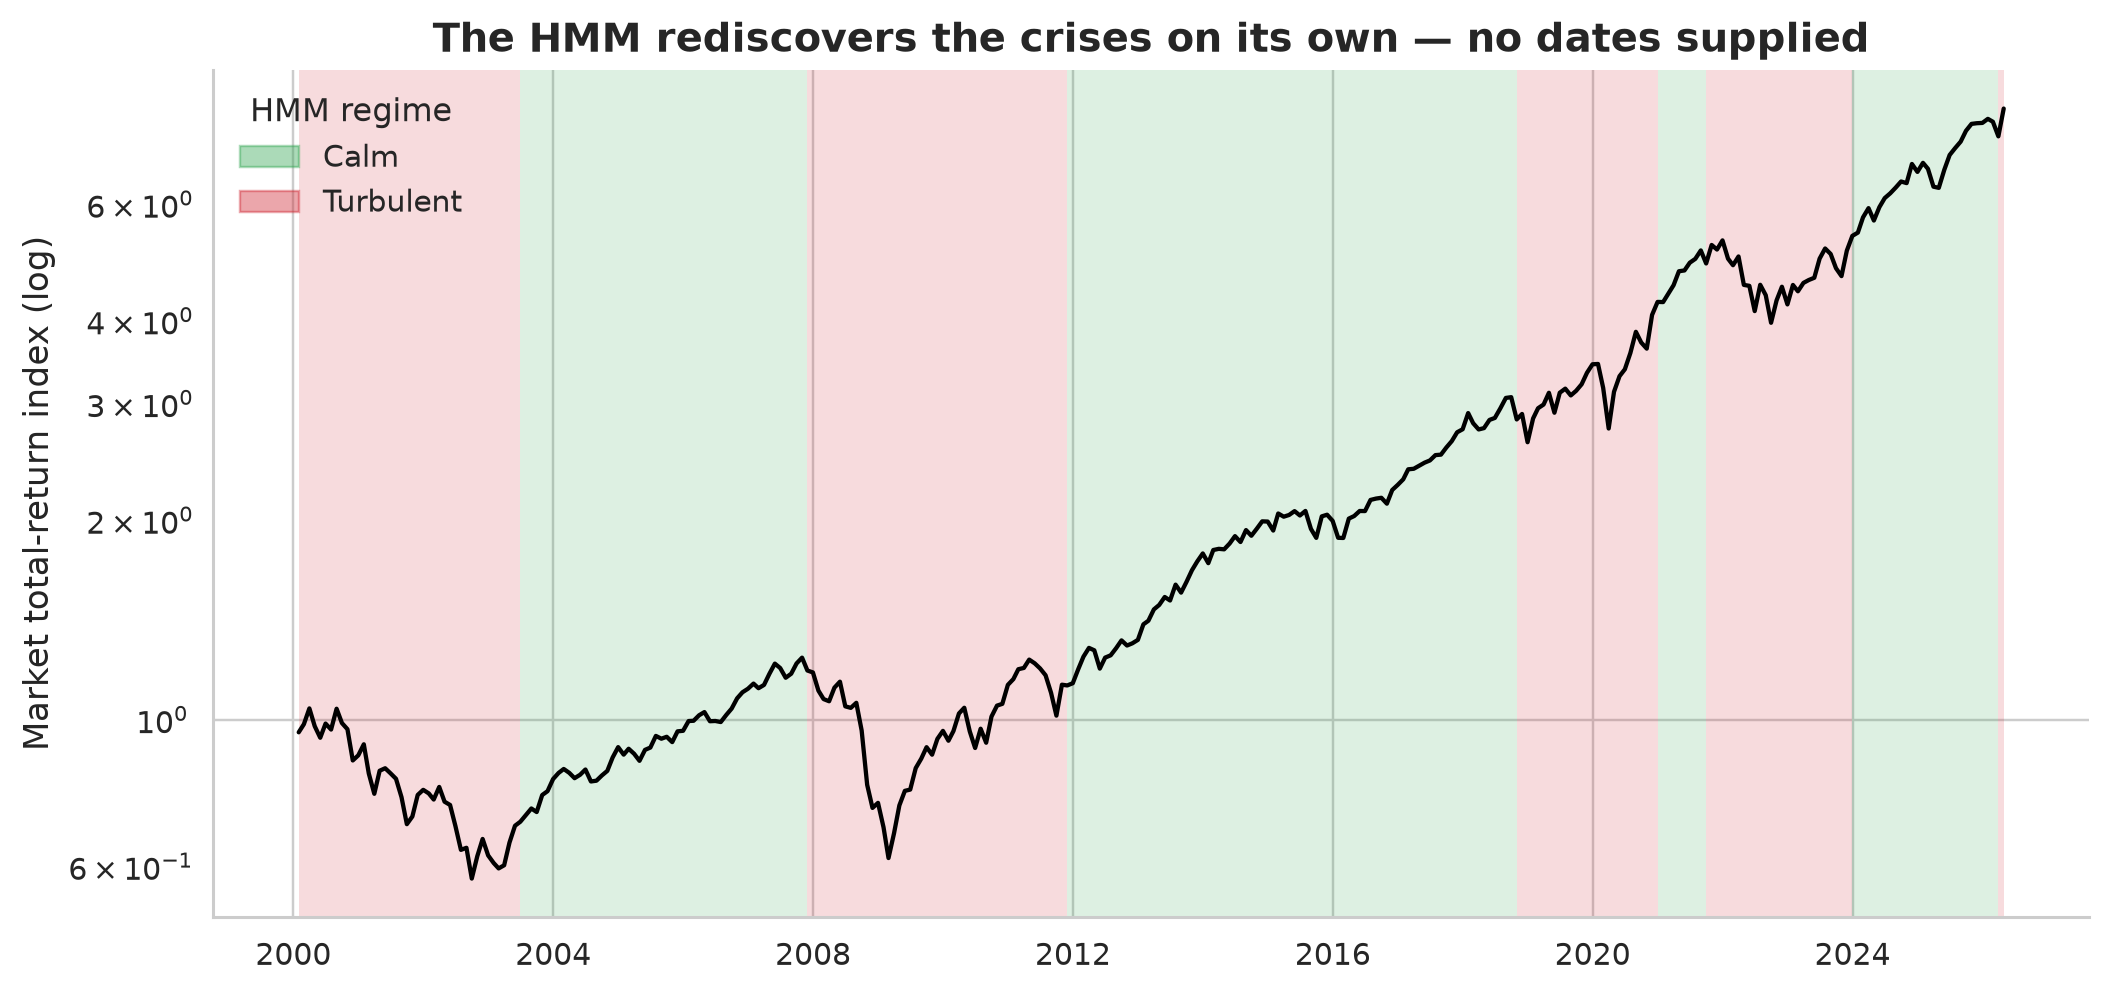
\includegraphics[width=0.96\textwidth]{fig07_regimes.png}
  \caption{Market total-return index (log) shaded by the smoothed HMM regime. The
  model rediscovers the crises on its own.}
  \label{fig:regimes}
\end{figure}

\begin{table}[htbp]
\centering
\caption{Estimated HMM regimes (states ordered by variance).}
\label{tab:regimestats}
\small
\begin{tabular}{rlrrrrr}
\toprule
state & label & n\_months & frequency & ann\_mean & ann\_vol & avg\_duration \\
\midrule
0 & Calm & 172 & 0.544 & 0.145 & 0.093 & 43.000 \\
1 & Turbulent & 144 & 0.456 & -0.010 & 0.208 & 28.800 \\
\bottomrule
\end{tabular}
\end{table}


Decomposing performance by regime (Table \ref{tab:regimedecomp},
Figure \ref{fig:decomp}) reveals the mechanism. In calm regimes the strategy
levers up and earns a higher return; in turbulent regimes it de-risks, cutting
volatility well below buy-and-hold. The risk-adjusted gain therefore comes from
two sources --- harvesting the premium more aggressively when it is safe to do
so, and protecting capital when it is not --- partly offset by missing some of
the most violent rebounds, which by construction occur in the turbulent state.

\begin{figure}[H]\centering
  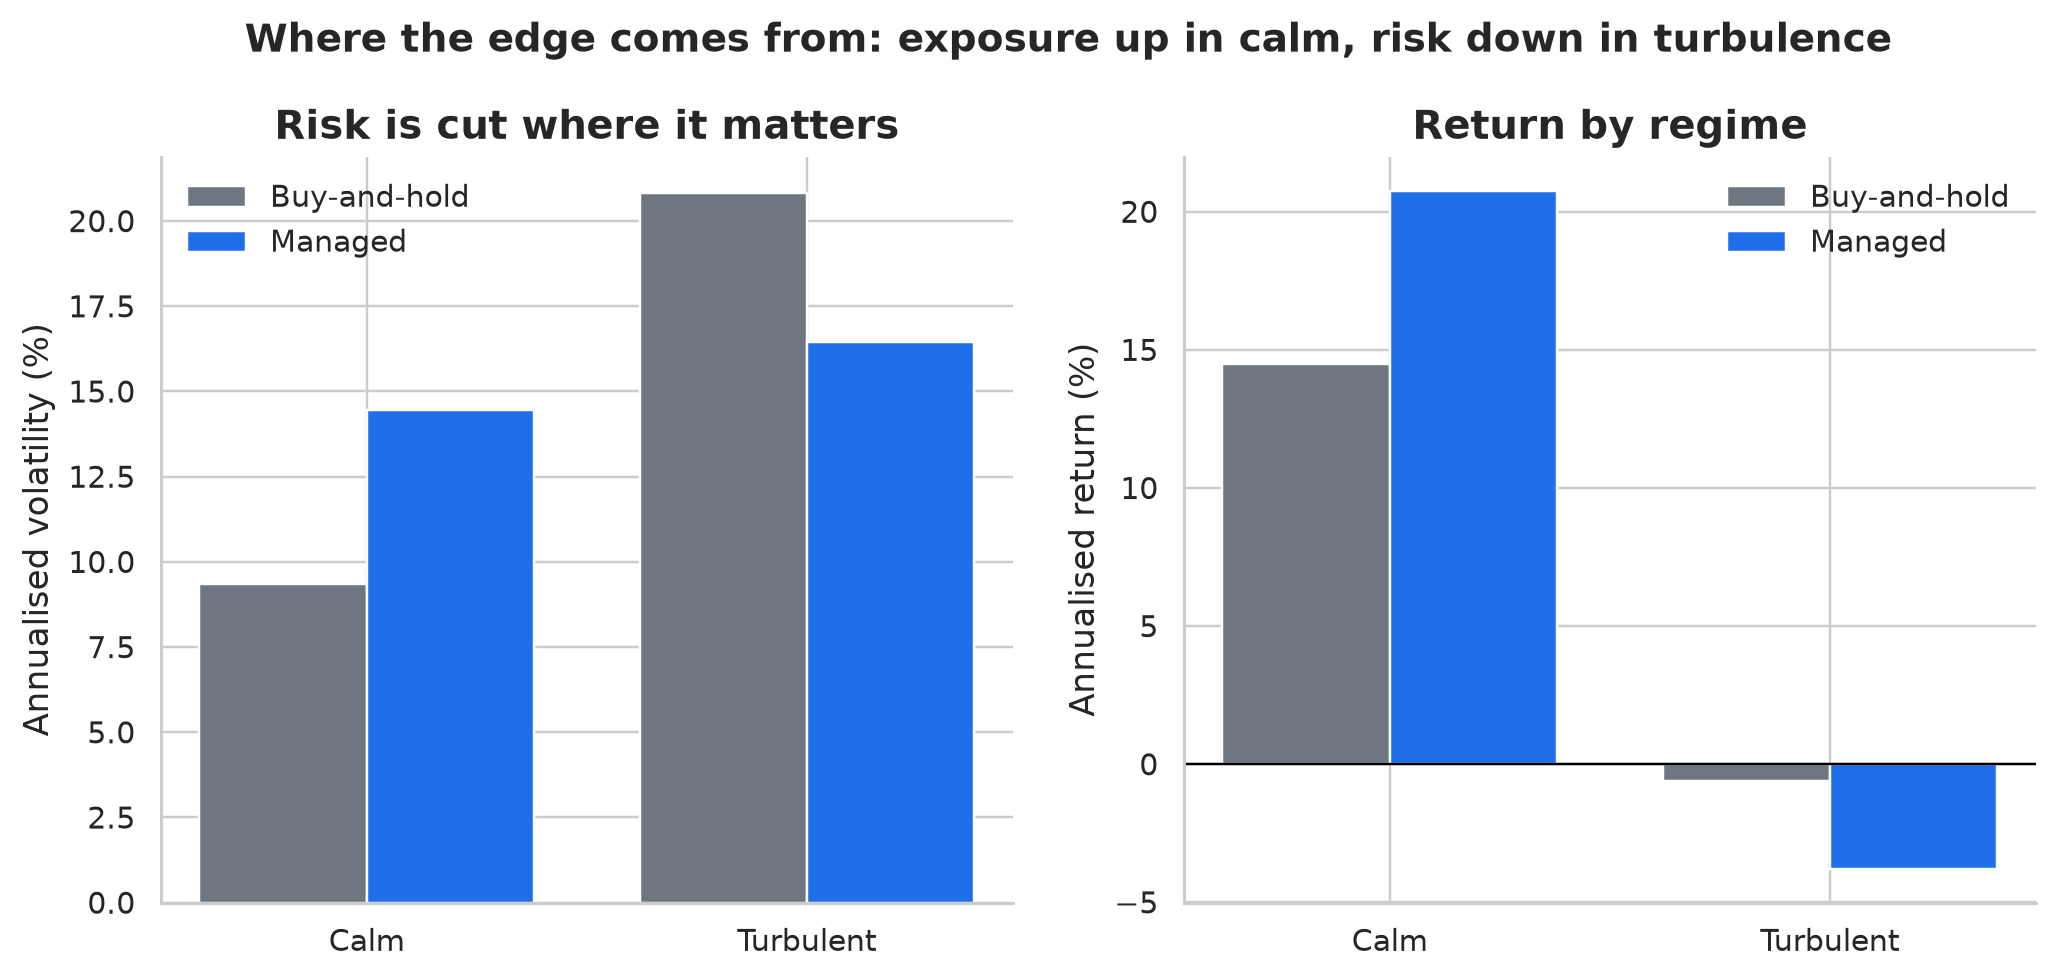
\includegraphics[width=0.96\textwidth]{fig08_regime_decomposition.png}
  \caption{Volatility and return by regime, managed vs.\ buy-and-hold.}
  \label{fig:decomp}
\end{figure}

\begin{table}[htbp]
\centering
\caption{Performance decomposition by (smoothed) regime.}
\label{tab:regimedecomp}
\small
\begin{tabular}{lrrrrrrrrr}
\toprule
regime & n\_months & frequency & avg\_exposure & mm\_ann\_return & bh\_ann\_return & mm\_ann\_vol & bh\_ann\_vol & monthly\_outperf & share\_of\_total\_outperf \\
\midrule
Calm & 172 & 0.546 & 1.588 & 0.207 & 0.145 & 0.144 & 0.093 & 0.005 & 1.733 \\
Turbulent & 143 & 0.454 & 0.864 & -0.038 & -0.006 & 0.164 & 0.208 & -0.003 & -0.733 \\
\bottomrule
\end{tabular}
\end{table}


% =========================================================================== %
\section{Multi-Asset Robustness and a Trend Overlay}

Two questions test whether the result is a principle or an artifact: does
volatility timing travel beyond the US market, and can we do better by
diversifying and adding a complementary signal? We assemble a USD total-return
panel of \nAssets{} assets across four classes --- six equity regions (US, UK,
Germany, Japan, France, emerging markets), Treasuries, gold, broad commodities,
and Bitcoin --- with excess returns over the same US risk-free rate. Their low
cross-correlations (Figure~\ref{fig:corr}) are the raw material for
diversification.

\textbf{Volatility timing alone does not travel uniformly}
(Table~\ref{tab:crossasset}, Figure~\ref{fig:crossasset}). It clearly helps US,
UK and Japanese equities but hurts several others (Germany, France, parts of
fixed income) --- consistent with the more sceptical out-of-sample evidence of
\citet{cederburg2020economic}. On its own it is largely an equity-index
phenomenon, and honesty requires saying so.

\textbf{The combination, however, is powerful.} Adding a time-series-momentum
overlay \citep{moskowitz2012time} --- long when the trailing twelve-month return
is positive, short otherwise, with the same volatility-managed sizing --- produces
statistically significant alpha across all six equity regions and commodities.
Combined into a diversified, inverse-volatility (risk-parity) portfolio, all
vol-matched to the diversified buy-and-hold benchmark (Table~\ref{tab:diversified},
Figure~\ref{fig:divequity}), the full system lifts the Sharpe ratio from
\sharpeDivBH{} to \sharpeDivTrend, cuts the maximum drawdown from \maxddDivBH{} to
\maxddDivTrend, and earns an annualised alpha of \alphaDivTrend{}
($t=\alphaDivTrendT$, Newey-West) --- comfortably more significant than the
single-market result, and \sharpeDivTrendNet{} on a Sharpe basis even after
\costBpsExt~bps of trading costs. The lesson is the standard one of quantitative
investing: the durable gains come from diversification and risk control, not from
a single secret signal.

\begin{figure}[H]\centering
  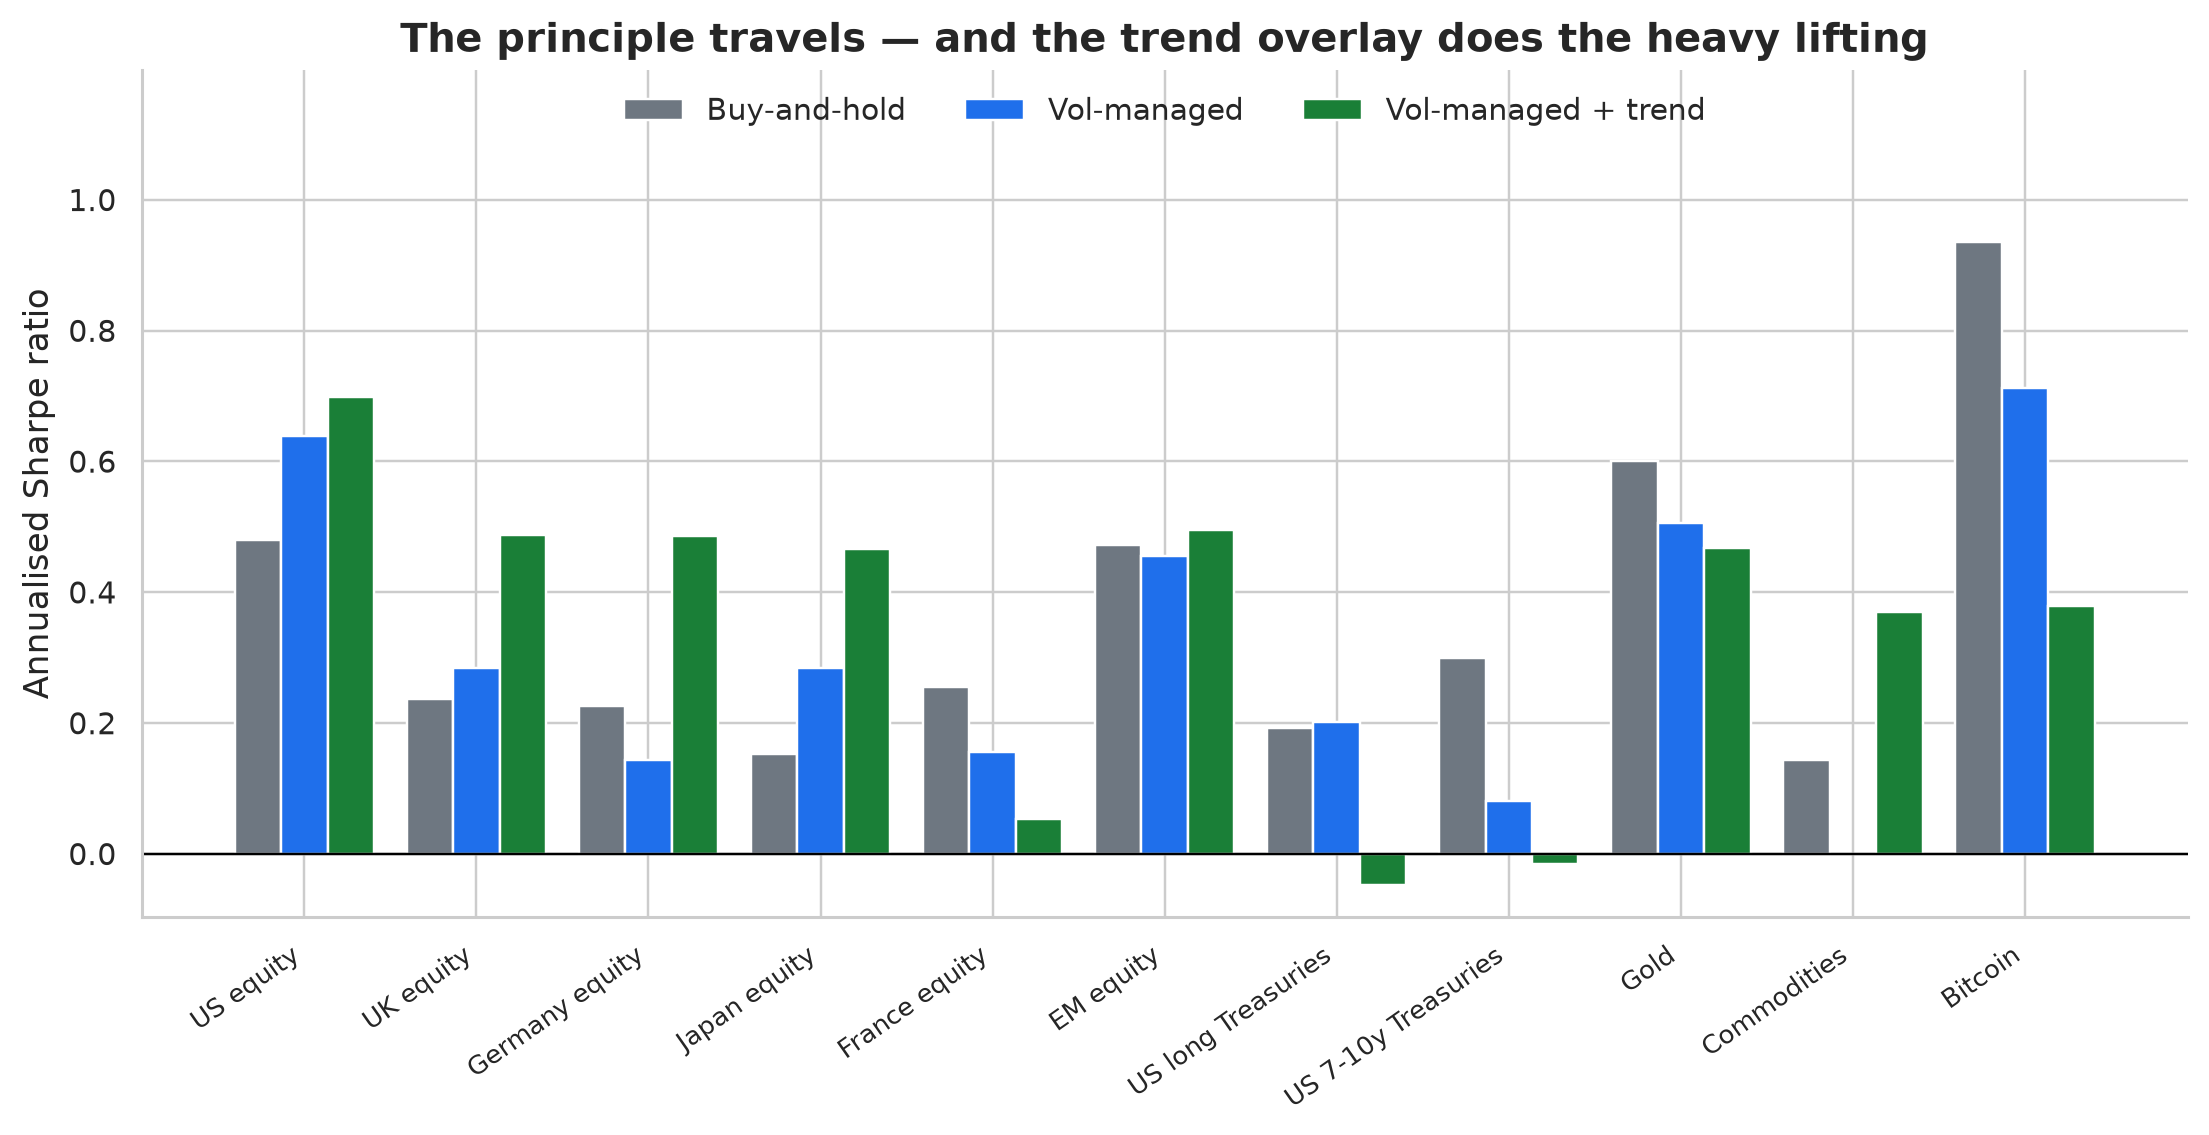
\includegraphics[width=0.92\textwidth]{fig09_cross_asset_sharpe.png}
  \caption{Sharpe ratios across the asset panel: buy-and-hold, volatility-managed,
  and volatility-managed with a trend overlay. Volatility timing alone is mixed;
  the trend overlay travels much more broadly.}
  \label{fig:crossasset}
\end{figure}

\begin{table}[htbp]
\centering
\caption{Volatility management and a trend overlay across assets (Sharpe ratios and managed-alpha $t$-statistics).}
\label{tab:crossasset}
\small
\begin{tabular}{llrrrrrr}
\toprule
asset & class & n\_months & BH SR & Managed SR & Mgd+Trend SR & Mgd alpha t & Trend alpha t \\
\midrule
US equity & Equity & 315 & 0.479 & 0.639 & 0.699 & 2.171 & 2.328 \\
UK equity & Equity & 315 & 0.236 & 0.284 & 0.487 & 0.781 & 2.320 \\
Germany equity & Equity & 315 & 0.226 & 0.143 & 0.486 & -0.269 & 2.265 \\
Japan equity & Equity & 315 & 0.152 & 0.284 & 0.466 & 1.453 & 2.130 \\
France equity & Equity & 315 & 0.255 & 0.156 & 0.054 & -0.347 & 0.168 \\
EM equity & Equity & 276 & 0.473 & 0.455 & 0.496 & 0.571 & 2.198 \\
US long Treasuries & Bonds & 284 & 0.193 & 0.201 & -0.048 & 0.394 & -0.455 \\
US 7-10y Treasuries & Bonds & 284 & 0.299 & 0.080 & -0.015 & -1.335 & -0.508 \\
Gold & Commodity & 257 & 0.600 & 0.506 & 0.468 & 0.120 & 1.248 \\
Commodities & Commodity & 242 & 0.144 & 0.000 & 0.371 & -0.753 & 1.546 \\
Bitcoin & Crypto & 139 & 0.936 & 0.713 & 0.378 & 0.004 & 0.557 \\
\bottomrule
\end{tabular}
\end{table}


\begin{figure}[H]\centering
  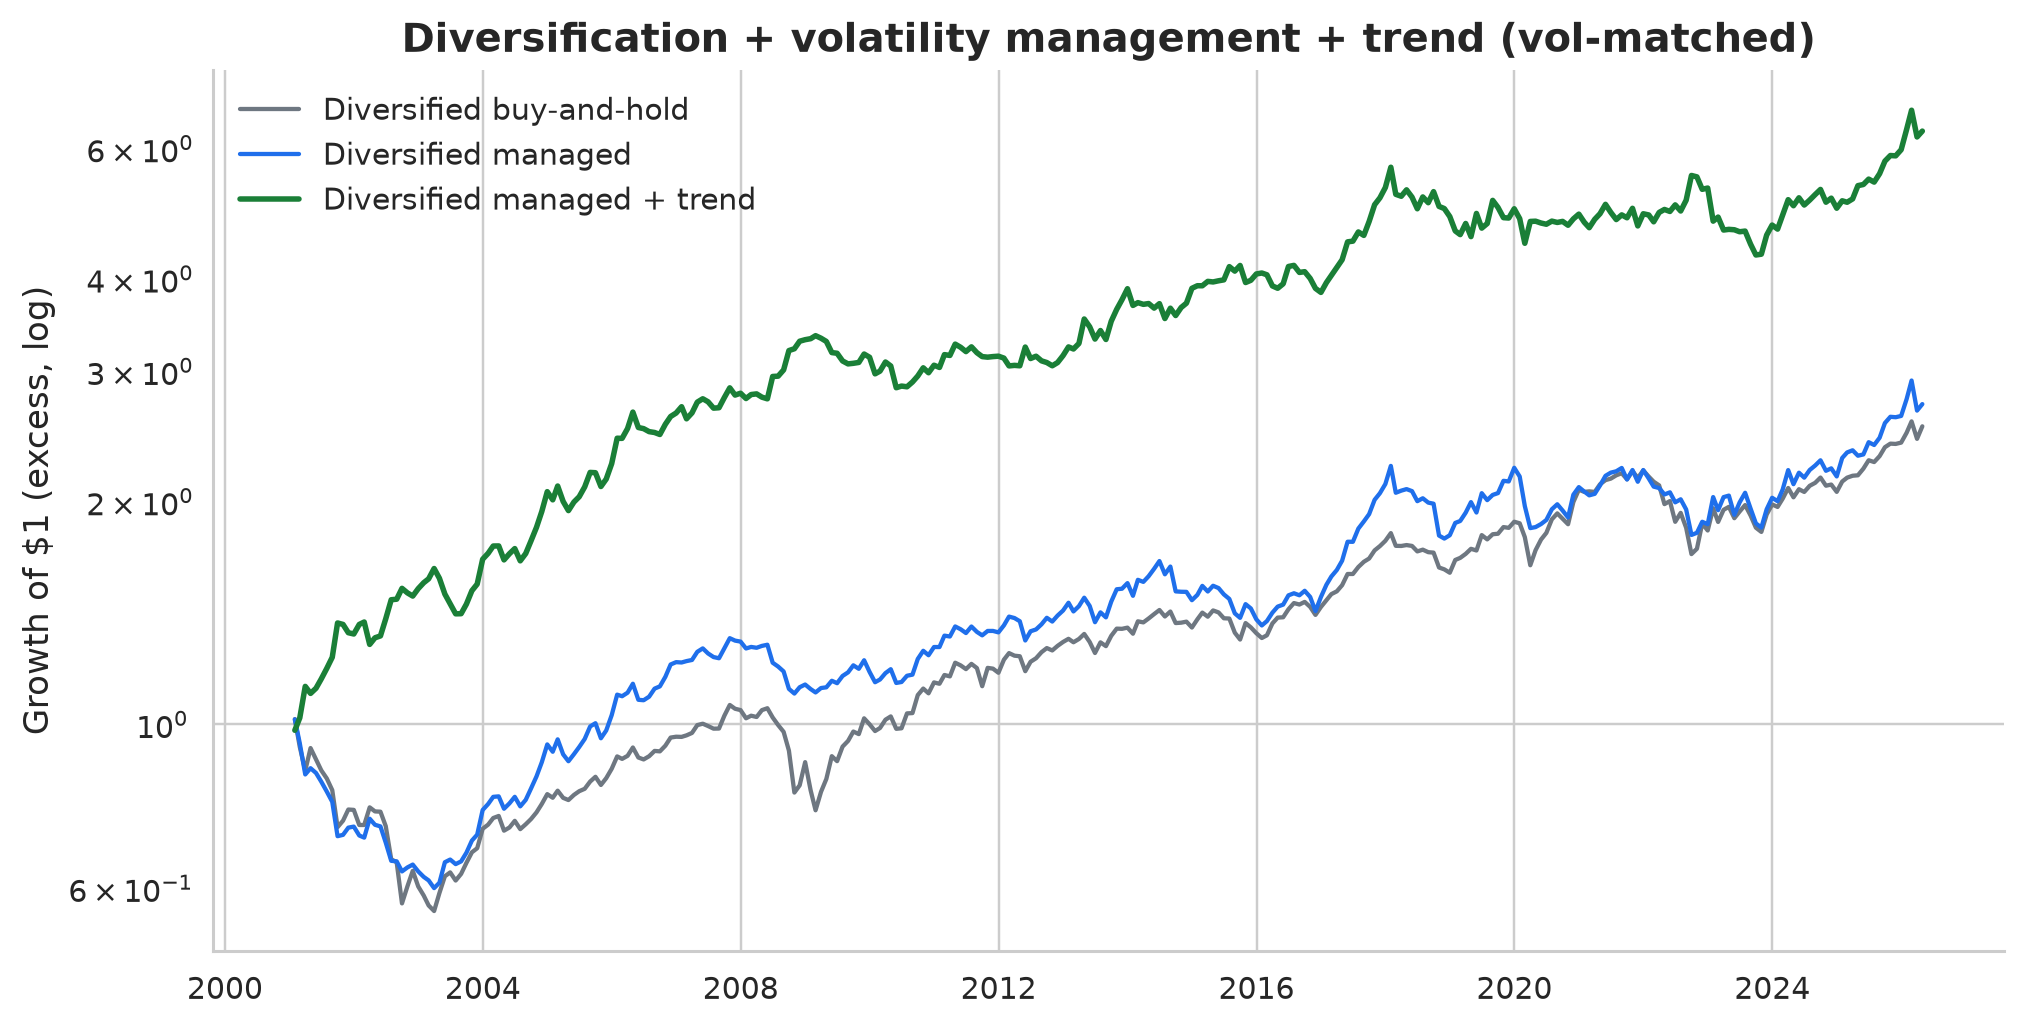
\includegraphics[width=0.9\textwidth]{fig10_diversified_equity.png}
  \caption{Diversified portfolios (excess growth of \$1, log scale), all
  vol-matched to the diversified buy-and-hold benchmark.}
  \label{fig:divequity}
\end{figure}

\begin{table}[htbp]
\centering
\caption{Diversified portfolios vs the single-market strategy (all vol-matched to the diversified buy-and-hold).}
\label{tab:diversified}
\small
\begin{tabular}{lrrrrrrr}
\toprule
strategy & ann\_return & ann\_vol & sharpe & max\_drawdown & sortino & alpha\_annual & alpha\_tstat \\
\midrule
US-only managed & 0.096 & 0.158 & 0.610 & -0.429 & 0.910 & 0.036 & 1.889 \\
Diversified buy-and-hold & 0.043 & 0.110 & 0.389 & -0.450 & 0.545 & -- & -- \\
Diversified managed & 0.046 & 0.110 & 0.413 & -0.409 & 0.595 & 0.010 & 0.796 \\
Diversified managed + trend & 0.079 & 0.110 & 0.719 & -0.239 & 1.214 & 0.080 & 3.630 \\
\bottomrule
\end{tabular}
\end{table}


\begin{figure}[H]\centering
  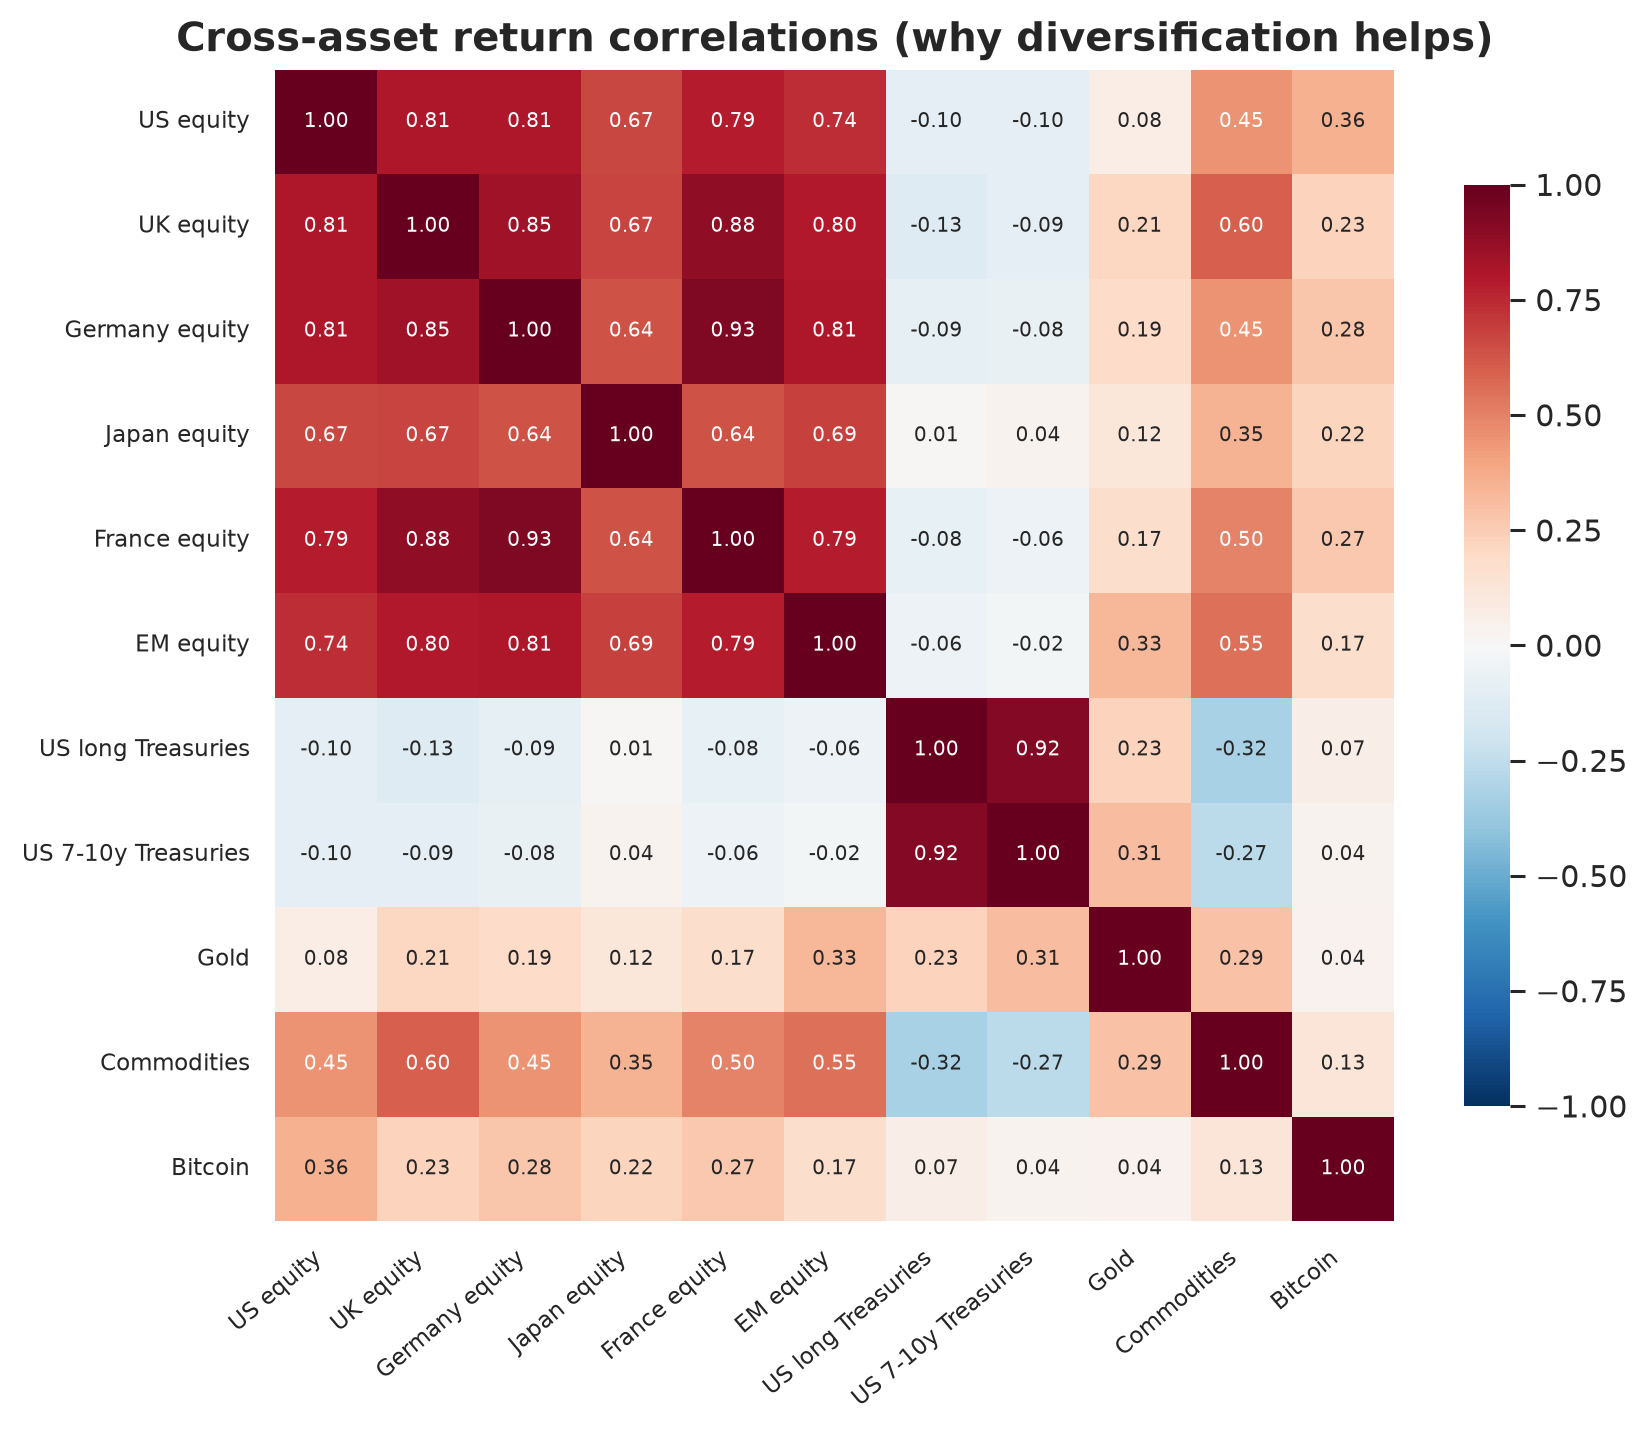
\includegraphics[width=0.66\textwidth]{fig11_correlation.png}
  \caption{Monthly excess-return correlations across the asset panel --- the
  source of the diversification benefit.}
  \label{fig:corr}
\end{figure}

% =========================================================================== %
\section{Discussion and Limitations}

The Deflated Sharpe Ratio of \deflatedSharpe{} (computed on the common evaluation
sample across the three forecasters tried) indicates the managed Sharpe ratio is
unlikely to be a multiple-testing artifact, even after correcting for
non-normality, sample length and the number of configurations searched. Several caveats remain. (i) A
backtest is not live trading: we model a turnover cost but ignore market impact,
financing spreads and the practical frictions of monthly rebalancing leverage.
(ii) Realized variance uses daily data; intraday data would sharpen both the HAR
model and the volatility proxy. (iii) Results are sample-dependent: the 2000--2026
window combines a secular decline in interest rates with two unusually fast
crashes, and the strategy's value is concentrated in turbulent regimes. (iv)
Capacity is finite and the leverage assumption is idealised. (v) The trend
overlay is itself a well-known, widely-traded signal, and the diversified result
depends on the chosen asset panel and on going short and using leverage in
practice. \emph{This is a research study and explicitly not investment advice.}

% =========================================================================== %
\section{Conclusion}

You cannot predict the price, but you can predict the risk --- and that is enough
to improve risk-adjusted returns. Replicating \citet{moreira2017volatility} on
the US market factor with strict out-of-sample discipline raises the Sharpe ratio
from \sharpeBH{} to \sharpeManaged{} (\sharpeBest{} with a GARCH forecaster on the
common sample), cuts drawdowns, survives realistic costs and a deflated-Sharpe
correction, and is
explained --- not merely reported --- by an unsupervised regime model that
rediscovers the crises and shows the strategy earning its keep by sizing risk to
the regime. Pushed across \nAssets{} assets and paired with a trend overlay in a
diversified portfolio, the same discipline reaches a Sharpe ratio of
\sharpeDivTrend{} with half the drawdown and an alpha significant at
$t=\alphaDivTrendT$ --- a reminder that in investing the reliable edges are
diversification and risk management, not the prediction of prices.

% =========================================================================== %
\bibliographystyle{plainnat}
\bibliography{references}

% =========================================================================== %
\clearpage
\appendix
\section{Plain-Language Summary (for non-specialists)}

\textbf{What problem are we solving?} Nobody can reliably say whether the stock
market will go up or down tomorrow --- that part really is close to a coin flip.
But there is something we \emph{can} see coming: how \emph{shaky} the market is
about to be. Calm weeks tend to be followed by calm weeks, and stormy weeks by
stormy weeks. Risk clusters together in time; direction does not.

\textbf{The idea, in one picture.} Think of driving a car. You cannot predict
every bend in the road ahead --- that is the \emph{price}. But you can feel when
the road turns icy --- that is the \emph{volatility}. A good driver does not try
to guess the bends; they simply \textbf{slow down on the ice and speed up when
the road is clear}. They arrive safer, and barely any later. This strategy does
exactly that with money: it invests \emph{more} when markets are calm and
\emph{less} when markets are turbulent, without ever trying to guess the
direction.

\textbf{Does it work?} Yes, in a careful and honest sense. At the \emph{same}
level of risk as simply holding the market, it earned a little more and ---
more importantly --- it fell much less during crashes (its worst loss was about
$-43\%$ instead of $-54\%$). The ride is smoother. We stress-tested it hard
(realistic trading costs, limits on borrowing, and a statistic that specifically
punishes results that could be down to luck), and it held up.

\textbf{But is it magic? No.} It is a respected, well-known professional
technique, not a money machine. Three honest caveats:
\begin{itemize}[leftmargin=1.4em,itemsep=0.15em]
  \item It does \emph{not} predict prices, so it will not make anyone rich
        quickly. It improves the \emph{quality} of returns (less stress, smaller
        crashes) more than it boosts their raw size.
  \item A test on past data is not a promise about the future. The advantage was
        real but modest over this period, and it depends on the era.
  \item Because the idea is well known, many investors already use it, which can
        slowly wear the advantage down.
\end{itemize}

\textbf{Where does it go from here?} The biggest, most reliable gains in investing
come from \emph{diversification} and \emph{risk control}, not from a secret
formula. We took exactly those steps: running the same risk-sizing idea across
\nAssets{} markets and asset classes at once (stocks around the world, bonds,
gold, commodities, even Bitcoin) and adding \emph{trend-following} --- simply
leaning with the wind, going with what has been rising and away from what has been
falling. Together, in a diversified portfolio, this nearly doubled the
risk-adjusted performance and roughly halved the worst loss. Importantly, even
this makes the system \emph{smoother and more robust} --- it is not a guaranteed
path to riches, and it relies on being able to short and to use leverage.

\textbf{The one-sentence takeaway.} You cannot predict the price, but you can
manage the risk --- and managing risk well is, over the long run, one of the few
things in investing that reliably pays off.

\end{document}
